% !TeX root = ../main.tex

\chapter{Methodology}
\label{ch:methodology}

This chapter describes the proposed token-level genomic foundation model classification framework. We present the overall system architecture, detail each component, and describe the training strategy, data pipeline, and evaluation methodology.

\section{System Overview}
\label{sec:method-overview}

\figref{fig:system-overview} illustrates the end-to-end pipeline. Given a raw DNA read of 150~bp, the system performs the following steps:
\begin{enumerate}
    \item \textbf{Tokenization}: The read is segmented into non-overlapping 6-mer tokens using the Nucleotide Transformer v2 tokenizer.
    \item \textbf{Token-level encoding}: The token sequence is processed by the pre-trained Nucleotide Transformer v2 backbone (with LoRA adapters), producing contextual embeddings for each token.
    \item \textbf{Attention pooling}: A multi-head attention pooling head aggregates the token embeddings into a fixed-dimensional classification vector.
    \item \textbf{Classification}: A feed-forward network maps the pooled representation to class logits.
\end{enumerate}

\begin{figure}[htbp]
\centering
\usetikzlibrary{arrows.meta, fit, positioning, shapes.geometric, backgrounds}
\resizebox{\textwidth}{!}{%
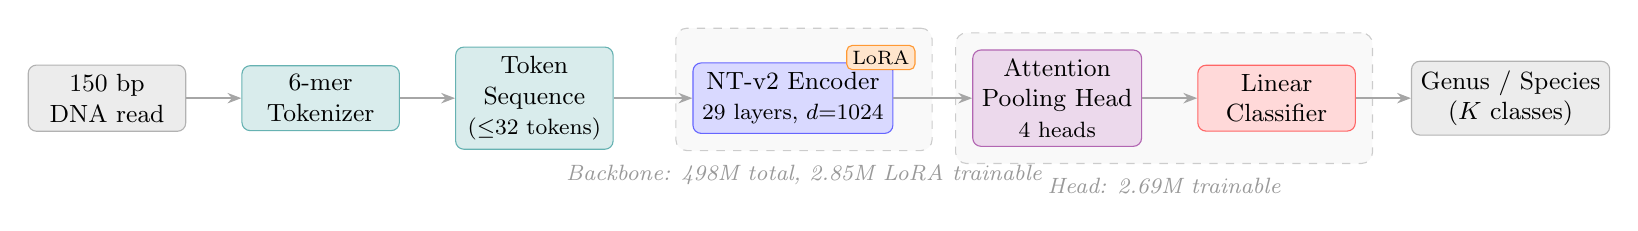
\begin{tikzpicture}[
    node distance = 0.55cm and 0.7cm,
    box/.style     = {draw, rounded corners=3pt, minimum width=2.0cm,
                      minimum height=0.7cm, align=center, font=\small,
                      fill=#1!15, draw=#1!60},
    arrow/.style   = {-{Stealth[length=5pt]}, thick, gray!70},
    label/.style   = {font=\footnotesize\itshape, text=gray!80},
    grpbox/.style  = {draw=gray!40, dashed, rounded corners=4pt,
                      inner sep=6pt, fill=gray!5},
]

%% Input
\node[box=gray]  (read)   {150 bp\\ DNA read};

%% Tokenizer
\node[box=teal,  right=of read]  (tok)    {6-mer\\ Tokenizer};

%% Token sequence
\node[box=teal,  right=of tok]   (tokens) {Token\\ Sequence\\ \footnotesize($\leq$32 tokens)};

%% NT-v2 encoder (with LoRA badge)
\node[box=blue,  right=1.0cm of tokens] (enc)   {NT-v2 Encoder\\ \footnotesize 29 layers, $d$=1024};
\node[draw=orange!80, fill=orange!20, rounded corners=2pt,
      font=\scriptsize, inner sep=2pt,
      above right=-0.1cm and -0.6cm of enc] (lora) {LoRA};

%% Attention pooling head
\node[box=violet, right=1.0cm of enc]  (pool)   {Attention\\ Pooling Head\\ \footnotesize 4 heads};

%% Classifier
\node[box=red,   right=of pool]  (clf)    {Linear\\ Classifier};

%% Output
\node[box=gray,  right=of clf]   (out)    {Genus / Species\\ ($K$ classes)};

%% Arrows
\draw[arrow] (read)   -- (tok);
\draw[arrow] (tok)    -- (tokens);
\draw[arrow] (tokens) -- (enc);
\draw[arrow] (enc)    -- (pool);
\draw[arrow] (pool)   -- (clf);
\draw[arrow] (clf)    -- (out);

%% Group: frozen backbone + LoRA
\begin{scope}[on background layer]
  \node[grpbox, fit=(enc)(lora)] (backbone_box) {};
\end{scope}
\node[label, below=0.05cm of backbone_box]
    {\textit{Backbone: 498M total, 2.85M LoRA trainable}};

%% Group: trainable head
\begin{scope}[on background layer]
  \node[grpbox, fit=(pool)(clf)] (head_box) {};
\end{scope}
\node[label, below=0.05cm of head_box]
    {\textit{Head: 2.69M trainable}};

\end{tikzpicture}%
}
\caption{Overview of the proposed token-level GFM classification pipeline. A 150~bp DNA read is tokenized into non-overlapping 6-mers, encoded by the LoRA-adapted NT-v2 backbone (29 layers, $d{=}1024$), aggregated via multi-head attention pooling, and classified into one of $K$ taxonomic classes (120 genera or 1,535 species). Orange badge indicates LoRA adapter modules; dashed boxes delineate the backbone and classification head parameter groups.}
\label{fig:system-overview}
\end{figure}

\section{Backbone: Nucleotide Transformer v2}
\label{sec:method-backbone}

We employ the \texttt{nucleotide-transformer-v2-500m-multi-species} model as the backbone encoder. This model is based on the ESM-2 architecture~\cite{Lin2023}, a protein language model architecture adapted for nucleotide sequences. The selection of NT-v2 over other genomic foundation models is motivated by four considerations:

\begin{enumerate}
    \item \textbf{Empirical performance on metagenomic reads}: A direct comparison of frozen-backbone baselines (Section~\ref{sec:exp-frozen}) shows that NT-v2 achieves 51.70\% genus-level accuracy, outperforming the 7B-parameter Evo-2 model~\cite{Brixi2025} (46.95\%) despite having 14$\times$ fewer parameters. This result provides direct empirical evidence that NT-v2's representations are better suited to metagenomic read classification.

    \item \textbf{Multi-species pre-training}: NT-v2's \texttt{multi-species} variant is pre-trained on 850 genomes spanning 174 species~\cite{DallaTorre2023}, making its pre-training distribution the closest among available GFMs to the multi-organism nature of metagenomic data. By contrast, DNABERT~\cite{Ji2021} is pre-trained exclusively on the human genome, which is taxonomically far from gut microbial sequences.

    \item \textbf{$k$-mer tokenization as a common ground with MetaTransformer}: MetaTransformer~\cite{Wichmann2023} demonstrates that $k$-mer-based sequence discretization is effective for metagenomic classification. NT-v2 shares this philosophy through its non-overlapping 6-mer tokenizer, establishing a direct methodological link. This allows the pre-trained 6-mer embeddings to serve as a principled initialization relative to MetaTransformer's learned-from-scratch 12-mer embeddings. DNABERT-2~\cite{Zhou2024dnabert2}, while multi-species, replaces $k$-mer tokenization with BPE, breaking this alignment.

    \item \textbf{Practical scalability}: At 498M parameters, NT-v2 can be fine-tuned with LoRA on a single H100 GPU with well under 10~GB of VRAM, making it feasible to run hundreds of training epochs over tens of millions of reads. Evo's 7B parameters~\cite{Nguyen2024}, while powerful for long-range genomic modeling, impose substantially higher memory requirements that are difficult to justify for 150~bp short-read classification.
\end{enumerate}

\subsection{Tokenization}

\paragraph{Stride and overlap.}
A $k$-mer tokenizer slides a window of length $k$ along a DNA sequence, converting each window into a vocabulary token. The \emph{stride} $s$ controls the step size between consecutive windows:

\begin{itemize}
    \item \textbf{Non-overlapping} ($s = k$): each nucleotide belongs to exactly one token.
          A 150~bp read yields $\lfloor 150 / k \rfloor$ tokens.
    \item \textbf{Overlapping} ($s = 1$): every nucleotide position starts a new token.
          A 150~bp read yields $150 - k + 1$ tokens.
\end{itemize}

For example, a 12-nucleotide sequence \texttt{AGTCGATTCGCA} tokenized with $k{=}6$ gives:

\begin{center}
\begin{tabular}{ll}
    \toprule
    Stride & Tokens \\
    \midrule
    $s{=}6$ (non-overlapping) & \texttt{AGTCGA} \quad \texttt{TTCGCA} \quad (2 tokens) \\
    $s{=}1$ (overlapping)     & \texttt{AGTCGA}, \texttt{GTCGAT}, \texttt{TCGATC}, \ldots \quad (7 tokens) \\
    \bottomrule
\end{tabular}
\end{center}

Table~\ref{tab:tokenization-counts} summarises the resulting token counts for a 150~bp read under the configurations used in this thesis.

\begin{table}[htbp]
    \centering
    \caption{Token counts for a 150~bp read under different $k$-mer tokenization settings.}
    \label{tab:tokenization-counts}
    \begin{tabular}{cccc}
        \toprule
        $k$ & Stride $s$ & Overlap & Tokens/read \\
        \midrule
        6  & 6 & Non-overlapping & 25 \\
        6  & 1 & Overlapping     & 145 \\
        12 & 12 & Non-overlapping & 12 \\
        12 & 1  & Overlapping     & 139 \\
        \bottomrule
    \end{tabular}
\end{table}

\paragraph{NT-v2 tokenization.}
The NT-v2 tokenizer uses non-overlapping 6-mers ($k{=}6$, $s{=}6$), the setting used during its pre-training. For a 150~bp read this produces 25 tokens (plus \texttt{[CLS]} and \texttt{[EOS]} special tokens). The maximum sequence length is set to 128 tokens, accommodating reads up to $\sim$768~bp with padding. Section~\ref{sec:exp-tokenization} presents a controlled ablation that quantifies the effect of different tokenization settings on classification accuracy.

\paragraph{Encoder Architecture}

The backbone consists of 29 Transformer encoder layers, each with:
\begin{itemize}
    \item Multi-head self-attention with 16 heads and hidden dimension 1,024.
    \item A feed-forward network (FFN) with intermediate dimension 4,096.
    \item Pre-layer normalization (LayerNorm before attention and FFN).
    \item Rotary position embeddings (RoPE)~\cite{Su2024} for encoding positional information.
\end{itemize}

The backbone outputs a tensor $H \in \mathbb{R}^{B \times T \times 1024}$, where $B$ is the batch size and $T$ is the sequence length. We use the \emph{full token sequence} (excluding special tokens) as input to the classification head, rather than extracting only the \texttt{[CLS]} token or applying mean pooling.

\subsection{LoRA Adaptation}
\label{sec:method-lora}

We apply LoRA~\cite{Hu2022} to the query ($W_Q$), key ($W_K$), and value ($W_V$) projection matrices in each of the 29 self-attention layers. The LoRA configuration is:

\begin{table}[htbp]
    \centering
    \caption{LoRA hyperparameters.}
    \label{tab:lora-config}
    \begin{tabular}{lr}
        \toprule
        \textbf{Parameter} & \textbf{Value} \\
        \midrule
        Rank $r$ & 16 \\
        Scaling factor $\alpha$ & 32 \\
        Dropout & 0.05 \\
        Target modules & $W_Q$, $W_K$, $W_V$ \\
        \midrule
        Trainable LoRA params & 2,850,816 \\
        Classification head params & 2,688,632 \\
        Total trainable params & 5,539,448 (1.11\%) \\
        Total model params & 498,623,561 \\
        \bottomrule
    \end{tabular}
\end{table}

Gradient checkpointing is enabled for the backbone to reduce peak GPU memory usage at the cost of recomputing activations during the backward pass.

\section{KmerFormer: A From-Scratch $k$-mer Transformer}
\label{sec:method-shallow}

The comparisons in this thesis require a model in which the factors under study are free to move. NT-v2's tokenizer is fixed by its pre-training and MetaTransformer is fixed at one encoder block over one vocabulary, so neither can be used to ask what depth is worth, what a longer $k$-mer is worth, or what an approximate vocabulary costs. We therefore build \textbf{KmerFormer}, a $k$-mer transformer trained from scratch in which the tokenizer, the stride, the vocabulary and the encoder depth are all configuration parameters under one training recipe. Arms that differ in one of them remain comparable, which is what makes the ablations of Chapter~\ref{ch:experiments} controlled.

\subsection{Architecture}

A read is tokenized into $k$-mers at a chosen stride, embedded, given a learned positional encoding, encoded by a pre-norm transformer stack, and pooled by the same attention-pooling head used with NT-v2 before a linear classifier:

\begin{itemize}
    \item \textbf{Token embeddings}: a randomly initialized matrix $E \in \mathbb{R}^{V \times d_{\text{model}}}$, where $V$ is the realized vocabulary of the chosen tokenizer ($V = 4{,}107$ for the NT-v2 6-mer scheme) and $d_{\text{model}} \in \{64, 128\}$.
    \item \textbf{Learned positional embeddings}: $P \in \mathbb{R}^{L_{\max} \times d_{\text{model}}}$, added to the token embeddings. Learned rather than sinusoidal encodings cannot extrapolate beyond trained positions, but every read here is 150~bp and yields a fixed token count, so the extrapolation is not needed and the additional freedom is obtained at no cost.
    \item \textbf{Pre-norm transformer encoder}: $N \in \{1, 8, 16, 29\}$ layers, 2 attention heads, $d_{\text{ff}} = 512$, GELU activation, dropout $p = 0.1$. Pre-norm placement leaves the residual path uninterrupted, which is what allows the deeper arms to train stably; MetaTransformer's post-norm arrangement normalises on the residual path itself and is a plausible reason its design does not extend past one layer.
    \item \textbf{Classification head}: the same 4-head attention-pooling head as the NT-v2 pipeline, with the input dimension matched to the encoder output. A masked mean-pooling variant is available as an ablation.
\end{itemize}

Holding the head fixed across backbones ensures that a performance difference is attributable to the encoder and the tokenizer rather than to the read-out.

\begin{table}[htbp]
    \centering
    \caption{Backbone configurations compared in this thesis. KmerFormer's shaded quantities---tokenizer, vocabulary and depth---are the ones the experiments vary; the other two models fix them.}
    \label{tab:backbone-comparison}
    \resizebox{\linewidth}{!}{%
    \begin{tabular}{lccc}
        \toprule
        \textbf{Aspect} & \textbf{NT-v2 $+$ LoRA} & \textbf{KmerFormer} & \textbf{MetaTransformer} \\
        \midrule
        Tokenizer & 6-mer, fixed & $k \in \{6, 13\}$, free & $k \in \{6,12,13\}$ \\
        Stride & $k$ & $1$ or $k$, free & 1 \\
        Vocabulary & 4,107, fixed & exact or hashed & exact \\
        Encoder layers & 29, fixed & 1--29, free & 1 \\
        Hidden dimension & 1,024 & 64 or 128 & 64 \\
        Attention heads & 16 & 2 & 2 \\
        Feed-forward dim & 4,096 & 512 & 512 \\
        Norm placement & pre-norm & pre-norm & post-norm \\
        Positional encoding & rotary (RoPE) & learned & sinusoidal \\
        Pre-training & MLM, 850 genomes & none & none \\
        Trainable params & 5.5M of 498M & all & all \\
        \bottomrule
    \end{tabular}%
    }
\end{table}

\subsection{Hashed Long-$k$ Vocabularies}
\label{sec:method-hashing}

At $k = 6$ the vocabulary is small and the encoder dominates the parameter budget. At $k = 13$ the relationship inverts: the training pool realises 33{,}545{,}099 distinct canonical 13-mers, which at $d = 64$ is an 8~GiB embedding table and 24~GiB once a sparse Adam variant materialises its two dense moment buffers. Two practical consequences follow---the table exceeds a 24~GiB card, and because an enumerated table requires sparse gradients, which torch's DDP reducer rejects, it cannot be trained under data parallelism at all.

KmerFormer therefore supports an approximate vocabulary. Each $k$-mer is mapped through a MurmurHash3 64-bit finalizer with seed $s = 42$ into one of $B = 2^{22} = 4{,}194{,}304$ buckets:
\begin{equation}
    e(w) \;=\; E\!\left[\, h_s(w) \bmod B \,\right], \qquad E \in \mathbb{R}^{B \times d_{\text{model}}},
    \label{eq:hashed-vocab}
\end{equation}
where $w$ is a $k$-mer over $\{\mathrm{A,C,G,T}\}$. Collisions are accepted rather than resolved: two unrelated 13-mers sharing a bucket share an embedding, and the model must recover the distinction from context. At $d = 128$ the table is 2~GiB in place of 8~GiB, it trains under DDP, and its cost in accuracy is measured directly in Section~\ref{sec:exp-thirteenmer}.

One property of the hashed scheme matters for evaluation. The exact vocabulary is \emph{canonical}---a $k$-mer and its reverse complement share an entry---so reverse-complement test-time augmentation is arithmetically a no-op on that arm. The hashed scheme is not canonical, since the two strands hash to unrelated buckets, so RC TTA has something to correct. The two arms therefore make a controlled pair for interpreting RC-TTA gains (Section~\ref{sec:method-rc-tta}).

\section{Classification Head: Attention Pooling}
\label{sec:method-head}

The classification head aggregates the variable-length token sequence into a fixed-dimensional representation and maps it to class logits. We use a multi-head attention pooling mechanism inspired by Perceiver~\cite{Jaegle2021} and Set Transformer~\cite{Lee2019}.

\subsection{Architecture}

The attention pooling head consists of:

\begin{enumerate}
    \item \textbf{Learnable queries}: $h = 4$ attention heads, each with head dimension $d_k = d / h = 256$, where $d = 1024$ is the backbone hidden size. A single learnable query vector per head is stored as $Q \in \mathbb{R}^{h \times d_k}$.

    \item \textbf{Cross-attention}: The backbone token embeddings $H \in \mathbb{R}^{T \times d}$ are projected to keys and values with $W_K, W_V \in \mathbb{R}^{d \times d}$ (no down-projection) and split across heads. Each head $i$ performs scaled dot-product attention between its query and the per-head key/value slices $K_i, V_i \in \mathbb{R}^{T \times d_k}$:
    \begin{align}
        K &= H W_K, \quad V = H W_V \\
        \text{head}_i &= \text{softmax}\!\left(\frac{Q_i K_i^\top}{\sqrt{d_k}}\right) V_i, \quad i = 1, \ldots, h
    \end{align}

    \item \textbf{Aggregation}: The $h$ single-vector head outputs are concatenated, yielding a representation of dimension $h \cdot d_k = d = 1024$.

    \item \textbf{Feed-forward classifier}:
    \begin{equation}
        \text{LayerNorm}(d) \to \text{Linear}(d, 512) \to \text{GELU} \to \text{Dropout}(p) \to \text{Linear}(512, K)
    \end{equation}
    where $K$ is the number of classes.
\end{enumerate}

With $d = 1024$, $h = 4$, and $K = 120$ genera, the head comprises the query ($1{,}024$), the key/value projections $W_K, W_V$ with their biases ($2 \times (1{,}048{,}576 + 1{,}024)$), the LayerNorm ($2{,}048$), and the two classifier layers ($524{,}800 + 61{,}560$), totalling $2{,}688{,}632$ trainable parameters (Table~\ref{tab:lora-config}); the species head ($K = 1{,}535$) correspondingly comprises $3{,}414{,}527$.

The attention pooling mechanism enables the model to selectively focus on the most taxonomically informative tokens in the sequence, analogous to how a biologist might focus on specific conserved marker regions within a read to determine its taxonomic origin.

\paragraph{Alternative Heads}
\label{sec:method-alt-heads}

We also implemented two alternative classification heads for comparison:

\textbf{Mean Pool Head}: Averages all token embeddings along the sequence dimension, followed by the same feed-forward classifier. This serves as the baseline aggregation strategy.

\textbf{Transformer Pool Head}: Applies a single Transformer encoder layer on top of the backbone output before mean pooling, adding another level of self-attention. This explores whether an additional attention layer can compensate for simple mean pooling.

\section{Training Strategy}
\label{sec:method-training}

\subsection{Two-Phase Training}

We employ a two-phase training strategy to stabilize learning:

\textbf{Phase 1 --- Head-only warmup} (5 epochs): The backbone is completely frozen, and only the classification head parameters are trained. This phase initializes the head weights to produce meaningful gradients before the backbone is unfrozen, preventing early gradient noise from corrupting pre-trained representations.

\textbf{Phase 2 --- Joint fine-tuning} (up to 25--30 epochs): LoRA adapters in the backbone are unfrozen, and both the backbone (via LoRA) and the classification head are trained jointly. Differential learning rates are used: the backbone learning rate ($3 \times 10^{-5}$) is set lower than the head learning rate ($5 \times 10^{-4}$) to preserve pre-trained knowledge.

\subsection{Optimization}

The training procedure uses the following optimization configuration:

\begin{table}[htbp]
    \centering
    \caption{Training optimization hyperparameters.}
    \label{tab:training-config}
    \begin{tabular}{lr}
        \toprule
        \textbf{Parameter} & \textbf{Value} \\
        \midrule
        Optimizer & AdamW \\
        Backbone learning rate & $3 \times 10^{-5}$ \\
        Head learning rate & $5 \times 10^{-4}$ \\
        Weight decay & 0.02 \\
        LR scheduler & Cosine with linear warmup \\
        Warmup ratio & 10\% of total steps \\
        Gradient accumulation steps & 1--2 \\
        Mixed precision & bfloat16 \\
        \bottomrule
    \end{tabular}
\end{table}

\textbf{Mixed precision training}: We use bfloat16 automatic mixed precision (AMP) on NVIDIA H100 GPUs. The bfloat16 format provides the dynamic range of float32 with reduced precision, avoiding the gradient underflow issues that arise with float16 and class-weighted losses.

\textbf{Early stopping}: Training is halted when validation accuracy does not improve for 7 consecutive epochs, and the model with the highest validation accuracy is saved as the final checkpoint.

\subsection{Transfer Learning Across Experiments}

To facilitate progressive scaling from smaller to larger datasets, we implement a transfer learning mechanism (\texttt{--init\_from}) distinct from the training resumption mechanism (\texttt{--resume}).

\textbf{Resume} (\texttt{--resume}): Loads the full training state (model weights, optimizer state, epoch counter, learning rate scheduler) from a checkpoint, enabling continuation of the \emph{same} experiment after a job interruption (e.g., SLURM time limit).

\textbf{Transfer learning} (\texttt{--init\_from}): Loads only the model weights from a checkpoint for a \emph{new} experiment, resetting the epoch counter and optimizer state. Supports partial loading, automatically skipping parameters with shape mismatches (e.g., when the classification head dimension changes between genus and species models). Phase~1 warmup is skipped when using transfer learning, as the backbone is already adapted.

\section{Data Pipeline}
\label{sec:method-data}

\subsection{Reference Database and Taxonomy}

Reference genomes are drawn from the Human Gastrointestinal Reference genome database (HGR-UMGS)~\cite{Almeida2019}, comprising two sources merged at the genus level: the Human Gut Reference (HGR; \texttt{taxonomy\_hgr.tab}) and the Unified Human Gastrointestinal Genome--derived Metagenome-Assembled Genomes Survey (UMGS; \texttt{taxonomy\_umgs.tab}).
The database covers \textbf{1{,}535 genomes spanning 120 genera}; because the source taxonomy is provided only down to genus, each genome is treated as a distinct ``species'' and is identified by its genome ID (e.g., \texttt{11861\_6\_55}).
Read headers therefore encode the full label hierarchy as
\texttt{>lbl|species\_class|genome\_id|genus\_class|genus\_name},
which is parsed at load time to produce both 120-class genus and 1{,}535-class species labels.
The same database underlies MetaTransformer~\cite{Wichmann2023}, which simplifies cross-method comparison.

\subsection{A Second Catalogue: Soil}
\label{sec:method-soil}

A result obtained on one reference set may be a property of that set rather than of the task. We therefore build a second, independent catalogue from RefSoil~\cite{Choi2017refsoil}, a curated collection of soil isolate genomes, spanning \textbf{309 genera}---$2.6\times$ the gut label space, with a different taxonomic composition and no overlap in provenance. Reads are simulated with the identical ART protocol and balanced pools are built at the same 5M and 50M budgets, so the only thing that changes between the two environments is the catalogue itself. This supports the cross-environment check of Section~\ref{sec:exp-lowdata}: an interaction that reproduces on a catalogue with twice the genera and a different origin is a property of the data budget rather than of one reference set.

\subsection{ART Read Simulation}

Training data consists of simulated metagenomic short reads generated from these reference genomes using the ART Illumina simulator~\cite{Huang2012}, following the same simulation protocol as MetaTransformer~\cite{Wichmann2023}.
ART is invoked in paired-end mode with the HiSeq~2500 (HS25) error profile, 150~bp read length, and fragment-length distribution $\mathcal{N}(\mu = 400, \sigma = 50)$~bp.

To prevent dataset composition from being driven by genome-length differences, reads are generated under a \emph{coverage-normalised} schedule rather than a fixed-coverage schedule.
The longest reference genome is assigned a coverage factor of $3\times$, and shorter genomes are assigned proportionally higher coverage so that, in expectation, every genome contributes the same number of reads to the merged FASTA.
In practice, this yields per-genome read counts within a narrow band ($\sim\!260$--$410$ reads per genome) due to discretisation; the relative class composition is therefore determined by the number of genomes per genus rather than by total genus genome length.

\paragraph{Pipeline.}
The full pipeline executes in five stages:
\begin{enumerate}
    \item ART generates paired-end reads for each genome FASTA under the coverage-normalised schedule above.
    \item Per-genome FASTQ outputs are merged into a single FASTQ stream.
    \item The stream is split into 64 chunks for parallel FASTQ$\to$FASTA conversion and label injection.
    \item The chunks are concatenated and shuffled with \texttt{seq-shuf} to produce the unified \texttt{reads.fa} ($\sim\!47$~GB, $\sim\!258$M reads).
    \item Balanced subsampling (Section~\ref{sec:method-subsampling}) draws fixed-size subsamples (e.g., 50M, 5M, 500K) from \texttt{reads.fa}.
\end{enumerate}

\paragraph{Reproducibility audit.}
We conducted an explicit audit of randomness sources across the full pipeline.
The findings are summarised below.

\emph{Reproducible by construction.}
The balanced-subsampling stage (Section~\ref{sec:method-subsampling}) seeds Python's \texttt{random} module with \texttt{seed=42}, so all balanced subsamples (500K, 5M, 50M) used in this thesis are exactly reproducible from a given \texttt{reads.fa}.
The train/validation split is computed by sklearn's \texttt{train\_test\_split} with \texttt{random\_state=42} (Section~\ref{sec:method-data}), and is therefore also deterministic for a fixed input subsample.

\emph{Not bit-for-bit reproducible.}
ART is invoked without \texttt{--rndSeed}, so the underlying $\sim\!258$M-read \texttt{reads.fa} would differ between fresh runs in individual read positions and per-base error realisations, although its aggregate statistical properties (per-genome coverage, label distribution, read-length distribution) are reproducible by construction.
The training script likewise does not set \texttt{torch.manual\_seed}, \texttt{numpy.random.seed}, or \texttt{torch.cuda.manual\_seed\_all}; \texttt{torch.backends.cudnn.deterministic} is left at its default (\texttt{False}); and the PyTorch \texttt{DataLoader} is constructed without \texttt{worker\_init\_fn}, so each worker's \texttt{numpy} and \texttt{random} states are uncontrolled.
Resume from a checkpoint restores model weights, optimiser state, and learning-rate scheduler state, but does not restore the PyTorch / CUDA / NumPy / Python RNG states, so a run resumed after a SLURM 48-hour timeout is not bit-for-bit identical to a hypothetical uninterrupted run.

\emph{Empirical impact.}
We did not perform repeated multi-seed runs of the full 50M-scale experiments due to compute constraints, but the residual non-determinism above is expected to produce run-to-run variation on the order of $\pm 0.1$--$0.3$~pp in genus Top-1 accuracy, which is small relative to the effects discussed in this thesis ($+15.60$~pp depth, $+40.42$~pp tokenization) and comparable to the ones we report as null (RC augmentation 0.13~pp, pooling 0.18~pp).
We acknowledge this as a methodological limitation and a candidate target for tightening in any follow-up study.

\subsection{Balanced Subsampling}
\label{sec:method-subsampling}

The full training dataset contains 258M reads with a highly skewed distribution across species. To mitigate class imbalance and enable controlled data scaling experiments, we implement a balanced subsampling strategy:

\begin{enumerate}
    \item \textbf{Scan}: The full FASTA file is scanned to extract all read headers and their species labels.
    \item \textbf{Allocate}: A target number of reads per species is computed as $n_{\text{target}} = N_{\text{total}} / K_{\text{species}}$, where $N_{\text{total}}$ is the desired subsample size and $K_{\text{species}}$ is the number of species.
    \item \textbf{Cap and redistribute}: For species with fewer reads than $n_{\text{target}}$, all available reads are included. The deficit is redistributed proportionally among species with surplus reads.
    \item \textbf{Sample}: Reads are randomly selected within each species to meet the per-species allocation.
\end{enumerate}

This procedure produces near-perfectly balanced subsamples. For a 50M subsample from 1,535 species, each species contributes $32{,}573 \pm 445$ reads.

\paragraph{Reverse-Complement Augmentation}

During training, each read is replaced with its reverse complement with probability $p = 0.5$. This augmentation is applied on-the-fly during data loading, doubling the effective diversity of the training set without requiring additional storage.

\subsection{Data Splitting}

The balanced subsamples are split into training (90\%) and validation (10\%) sets at the \emph{read} level---i.e., individual reads from the same genome may appear in both the training and validation splits.
The split is stratified by species label so that every one of the 1{,}535 species is represented in both partitions and class proportions are preserved within each.
For the hierarchical evaluation of Section~\ref{sec:spv4-hierarchical-prelim}, an additional, fully disjoint test set is drawn from the MetaTransformer validation reads (\texttt{val\_reads.fa}); see Section~\ref{sec:spv4-data-leakage} for the data-leakage audit motivating this choice and for empirical evidence that read-level (rather than genome-level) splitting does not lead to detectable memorisation in this study.

\section{Evaluation Methodology}
\label{sec:method-eval}

\subsection{Metrics}

We evaluate classification performance using the following metrics:

\textbf{Micro accuracy} (overall accuracy): The fraction of correctly classified reads. This metric is dominated by abundant classes and reflects real-world performance on typical samples.

\textbf{Macro F1}: The unweighted average of per-class F1 scores. This metric weights all classes equally, providing a measure of performance across the full taxonomic diversity including rare taxa.

\textbf{Balanced accuracy}: The average of per-class recall, equivalent to macro recall.

\textbf{Top-$k$ accuracy}: The fraction of reads for which the correct class appears in the top $k$ predictions. We report top-3, top-5, and top-10 accuracy.

\textbf{F1$=$0 class count}: The number of classes with zero F1 score (i.e., classes for which the model makes no correct predictions). This directly measures the ``dead class'' problem.

\textbf{Train-validation gap}: The difference between training accuracy and validation accuracy, serving as a proxy for overfitting.

\subsection{Reverse-Complement Test-Time Augmentation}
\label{sec:method-rc-tta}

At inference, we employ RC TTA: each read is classified twice (forward and reverse complement), and the logits are averaged before applying softmax:
\begin{equation}
    \hat{y} = \arg\max_k \tfrac{1}{2}\left[ f_\theta(r) + f_\theta(\bar{r}) \right]
    \label{eq:rc-tta}
\end{equation}
where $f_\theta(r)$ and $f_\theta(\bar{r})$ are the logit vectors for the forward and reverse-complement reads, respectively. This ensembling exploits the biological strand symmetry of DNA and consistently improves accuracy.

\subsection{Off-Catalogue Evaluation: Track~A and the ANI Ladder}
\label{sec:method-offcat}

Held-out reads simulated from the reference genomes measure performance under complete reference coverage. Because real communities contain organisms the catalogue does not, we add two pools whose source genomes are absent from the training reference.

\textbf{Track~A (out-of-genome)} simulates one assembly per genus from RefSeq genomes not in the training catalogue: 595{,}000 reads reduced to 580{,}000 over 116 genera after removing three accessions found to overlap the training set. It guarantees unseen \emph{assemblies}, but mixes different strains of catalogued species with genuinely novel species under a single number.

\textbf{Track~B (ANI ladder)} separates the distances Track~A averages. Candidate genomes are stratified by skani average nucleotide identity to the closest reference genome, at the 95\% species boundary used for ANI-based species delineation in GTDB~\cite{Parks2022}, into three rungs: \textsc{strain} (a different strain of a species the reference holds), \textsc{species} (a different species of a represented genus), and \textsc{far} (no reference genome within reach). The same fourteen genera are held present at every rung, so a line drawn through the rungs measures distance rather than class count, and chance accuracy is 7.1\% at all three.

In both pools the label space is unchanged: every read comes from a genome whose genus is one of the 120 trained on, so the task remains a 120-way decision with a correct answer available and ``far'' names a distance rather than a missing label. Alongside accuracy we report \emph{retention}, the ratio of far-rung to strain-rung accuracy, which summarises how much of a model's closed-set performance survives the move away from the reference.

\subsection{Species-Level Evaluation Modes}
\label{sec:method-species-eval}

For species-level classification (1,535 classes), we introduce two additional evaluation modes to decouple the contributions of genus-level and intra-genus discrimination:

\textbf{Oracle-genus evaluation}: Given the \emph{true} genus label, the species logits are masked to only allow species belonging to that genus. This answers: ``Given perfect genus identification, how well can the model discriminate species within each genus?''

\textbf{Top-$k$ genus routing}: The genus classifier produces the top-$k$ genus predictions. The candidate species set is the union of all species belonging to these $k$ genera. Species logits are then masked to this candidate set. This simulates a realistic two-stage hierarchical classification pipeline.

\section{Computational Considerations}
\label{sec:method-compute}

\paragraph{Hardware}

All experiments are conducted on the TWCC (Taiwan Computing Cloud) SLURM cluster equipped with NVIDIA H100 80~GB HBM3 GPUs. The SLURM partition enforces a 48-hour maximum wall time per job, necessitating checkpoint-resume support for long training runs.

\paragraph{Memory Optimization}

Several techniques are employed to manage GPU memory:
\begin{itemize}
    \item \textbf{Gradient checkpointing}: Recomputes intermediate activations during the backward pass rather than storing them, trading $\sim$30\% additional compute for $\sim$60\% memory reduction.
    \item \textbf{Mixed precision (bfloat16)}: Reduces memory requirements for activations and gradients by approximately 50\% compared to float32.
    \item \textbf{LoRA}: Keeps the majority of backbone parameters frozen, reducing the optimizer state memory from $\sim$4$\text{GB}$ (full fine-tuning with AdamW) to $\sim$44$\text{MB}$.
\end{itemize}

\paragraph{Resource Monitoring}

To assess computational resource adequacy and identify bottlenecks, we implement a dedicated resource monitoring module that tracks:
\begin{itemize}
    \item GPU VRAM usage (PyTorch allocated, nvidia-smi total, and peak values).
    \item GPU compute utilization (sampled every 30 seconds via nvidia-smi).
    \item System RAM usage (process RSS and peak).
    \item Per-epoch wall-clock time and throughput (reads per second).
\end{itemize}
These metrics are logged to \texttt{training\_history.csv} and a comprehensive \texttt{resource\_report.json} at the end of training.

\section{Summary}

This chapter has described the complete methodology for token-level GFM classification of metagenomic reads. The framework combines a pre-trained Nucleotide Transformer v2 backbone with LoRA adaptation, an attention-pooling classification head, two-phase training with transfer learning support, balanced subsampling, and RC augmentation. The evaluation methodology encompasses multiple metrics at both genus and species levels, with specialized evaluation modes for dissecting hierarchical classification performance.
